\section{Nguyên lý}
Đối với hầu hết chúng ta, không thể thăm dò cấu trúc mạng của Internet một cách trực tiếp. Tuy nhiên, chúng ta có thể dễ dàng khám phá đường dẫn cụ thể được thực hiện bởi các gói dữ liệu di chuyển giữa máy tính của chúng ta (hoặc bất kỳ máy tính nào chúng ta có quyền truy cập) và hầu hết các đường dẫn khác trên Internet. Công cụ để làm điều này được gọi là traceroute.\par
Ngoài một địa chỉ đích, cho biết nơi đến, mỗi gói Internet cũng chứa một địa chỉ nguồn, cho biết nơi bắt đầu và thời gian tồn tại (TTL). TTL là một số chỉ định số lượng tối đa các bước nhảy tối đa mà gói có thể thực hiện để đến đích của nó, một bước nhảy là sự truyền tải của một cạnh trong mạng. Tại mỗi bước nhảy, TTL bị giảm đi một, và nếu nó đạt đến 0 thì gói bị loại bỏ, nghĩa là nó bị xóa và không được chuyển tiếp qua mạng nữa. Nếu chúng ta đang sử dụng TCP, một tin nhắn cũng sẽ được gửi lại cho người gửi để thông báo cho họ rằng gói tin đã bị loại bỏ và nơi nó đến (Đây là một phần trong cơ chế của TCP để đảm bảo việc truyền dữ liệu đáng tin cậy). TTL tồn tại chủ yếu như một biện pháp bảo vệ để ngăn chặn các gói tin bị mất trên Internet và lang thang mãi, ngoài ra chúng ta cũng có thể sử dụng nó để theo dõi tiến trình hoạt động của gói. Ý tưởng là như sau.\par
Đầu tiên, chúng tôi gửi một gói TCP có địa chỉ đích của đỉnh mạng mà chúng tôi quan tâm và chỉ số TTL là 1. Gói này thực hiện một bước nhảy đến bộ định tuyến đầu tiên trên đường đi, TTL của nó giảm xuống 0, gói bị loại bỏ bởi bộ định tuyến và một thông báo được gửi lại cho chúng tôi, cho biết địa chỉ IP của bộ định tuyến. Chúng tôi ghi lại địa chỉ này và sau đó lặp lại quy trình với chỉ số TTL là 2. Lần này gói tạo ra hai bước trước khi bị loại bỏ và thông báo trả về cho chúng tôi biết địa chỉ IP của bộ định tuyến thứ hai. Quá trình được lặp lại với những TTL lớn hơn cho đến khi đạt đến đích và ta thu được tập hợp địa chỉ IP xác định tuyến đường được thực hiển chuyển gói. Có các công cụ phần mềm sẽ tự động thực hiện toàn bộ quy trình trên và in ra danh sách các địa chỉ IP cho chúng tôi. Trên hầu hết các máy tính, công cụ thực hiện việc này được gọi là traceroute.\par
Chúng ta có thể sử dụng traceroute (hoặc một công cụ tương tự) để thăm dò cấu trúc mạng của Internet. Ý tưởng là tập hợp một tập hợp dữ liệu các đường dẫn theo dõi giữa nhiều cặp điểm khác nhau trên Internet. Nếu may mắn, hầu hết các cạnh trong mạng (mặc dù thường không phải tất cả chúng) sẽ xuất hiện ít nhất một lần trong tập hợp này và liên kết của tất cả chúng sẽ đưa ra một bức tranh hoàn chỉnh hợp lý về mạng. Ở các nghiên cứu ban đầu, vì mục đích nhanh chóng, ta chỉ giới hạn một số máy tính nguồn, nhưng gần đây, dự án DIMES sử dụng bộ sưu tập hàng ngàn nguồn để phát triển một bức tranh hoàn chỉnh về mạng.\par
Các đường dẫn từ bất kỳ nguồn đơn lẻ nào đến một tập hợp đích tạo thành một cấu trúc hiển thị dạng sơ đồ cây như Hình \ref{fig:h22} (a), (b) và (c). Các máy tính nguồn nên được phân phối tốt qua mạng. Nếu chúng ở gần nhau, thì có thể có sự chồng chéo đáng kể giữa các đường theo dõi đến các đỉnh xa, điều đó có nghĩa là chúng sẽ nhân đôi không cần thiết, thay vì trả về các phép đo độc lập.\par

\begin{figure}[ht]
\centering
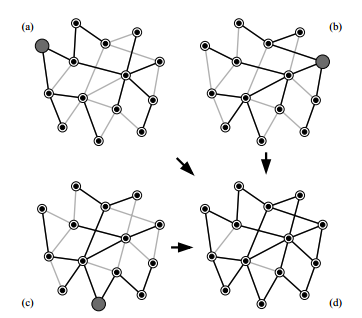
\includegraphics[width=0.5\textwidth]{res/h22.png}
\caption{Tái thiết lập cấu trúc Internet từ kết quả theo dõi: Trong các bảng (a), (b) và (c), ta hiển thị in đậm các cạnh trong ba bộ đường theo dõi bắt đầu đỉnh được tô sáng. Trong bảng điều khiển (d) ta tạo thành sự kết hợp của (a) (b) và (c) để tạo thành một bức tranh về cấu trúc liên kết mạng tổng thể. Lưu ý rằng một vài cạnh bị thiếu trong ảnh(các cạnh màu xám còn lại trong bảng (d)) bởi vì tình cờ chúng không xuất hiện trong bất kỳ ba bộ dữ liệu theo dõi (a) (b) (c).}
\label{fig:h22}
\end{figure}

\section{Cấu trúc Internet}
Khi một người có một tập hợp dữ liệu theo dõi phù hợp, một liên kết đơn giản của tất cả các đường dẫn xuất hiện trong tập dữ liệu sẽ cho chúng ta ảnh chụp nhanh về cấu trúc mạng (Hình \ref{fig:h22} d). Ta đi qua từng đường dẫn và ghi lại đỉnh cho mọi địa chỉ IP xuất hiện trong đường dẫn và cạnh giữa mỗi cặp địa chỉ. Không có khả năng một quy trình như vậy sẽ tìm thấy tất cả các cạnh trong mạng (xem lại hình \ref{fig:h22}d) và đối với các nghiên cứu dựa trên số lượng nguồn nhỏ có thể có sự sai lệch khá nghiêm trọng trong việc lấy mẫu các cạnh . Tuy nhiên, các bộ dữ liệu tốt hơn đang trở nên khả dụng theo thời gian, và người ta tin rằng ta đã đang có một bức tranh hoàn chỉnh hợp lý về hình dạng của Internet.\par
Trên thực tế, hiếm khi có thể thực hiện ghi lại mọi địa chỉ IP trên Internet dưới dạng một đỉnh riêng biệt. Có khoảng 2 tỷ địa chỉ IP được sử dụng trên Internet cùng một lúc, với nhiều địa chỉ xuất hiện và biến mất khi máy tính được bật, tắt hoặc kết nối được hay không được với Internet. Hầu hết các nghiên cứu về Internet đều bỏ qua các máy tính của “người dùng cuối” (End users) và chỉ giới hạn ở các bộ định tuyến, tập trung vào các vùng bên trong và bỏ qua phần ngoài cùng (Hình 2.1). Ở đây ta đề cập đến các Internet như vậy với các đại diện ở cấp độ bộ định tuyến. Các đỉnh trong mạng là các bộ định tuyến và các cạnh giữa chúng là các kết nối mạng.\par
Có vẻ lạ khi bỏ qua các máy tính của người dùng cuối, vì suy cho cùng, họ là toàn bộ lý do cho sự tồn tại của Internet. Tuy nhiên, cấu trúc của mạng ở cấp bộ định tuyến mới chịu trách nhiệm cho hầu hết các khía cạnh về hiệu suất, độ mạnh và hiệu quả của mạng, điều khiển các mô hình lưu lượng trên mạng và tạo thành trọng tâm của hầu hết công việc về cấu trúc và thiết kế Internet, và đó mới là những vấn đề được khoa học quan tâm. Do đó, việc tập trung vào cấu trúc cấp bộ định tuyến là điều hợp lý.\par
\section{Phân nhóm địa chỉ}
Ngay cả sau khi xóa tất cả hoặc hầu hết các máy tính của người dùng cuối khỏi mạng, cấu trúc mạng ở cấp bộ định tuyến vẫn còn quá chi tiết. Thông thường ta muốn một đại diện chi tiết hơn của mạng cung cấp cho ta một bức tranh tổng thể rộng hơn về cấu trúc mạng. Các biểu diễn như vậy được tạo bằng cách nhóm các nhóm địa chỉ IP lại với nhau thành các đỉnh đơn. Ba cách phổ biến để phân nhóm địa chỉ dựa trên ba cách biểu diễn chi tiết khác nhau, ở cấp độ của mạng con, miền và hệ thống tự trị. (subnets, domains, and autonomous systems)\par
Mạng con (subnets) là một nhóm các địa chỉ IP được xác định như sau. Địa chỉ IP bao gồm bốn số, mỗi số trong phạm vi từ 0 đến 255 (8 bit nhị phân) và thường được viết trong một chuỗi, cách nhau bởi dấu chấm. Một khối địa chỉ gồm bốn khối nhỏ dạng “xxx”. Khối cuối là mạng con lớp C, tiếp theo là lớp B và lớp A.\par
Cấp độ cao hơn mạng con là cấp độ miền (domains). Miền là một nhóm máy tính và bộ định tuyến, thông thường kiểm soát bởi một tổ chức và được xác định bởi một tên miền duy nhất, thường là hai hoặc ba phần cuối của địa chỉ máy tính khi được viết dưới dạng văn bản con người có thể đọc. Ví dụ .hust.edu.vn là tên miền của trường Đại họa Bách Khoa Hà Nội. Tên miền của máy tính được xác định một cách đơn giản từ địa chỉ IP của máy tính bằng cách tra cứu DNS, một dịch vụ mạng được thiết lập để cung cấp loại thông tin này. Do đó, với cấu trúc liên kết mạng cấp bộ định tuyến, việc xác định miền mà mỗi bộ định tuyến thuộc và các đỉnh trong mạng theo tên miền là một nhiệm vụ đơn giản.\par
Cấp độ thứ ba là hệ thống tự trị (autonomous systems). Một hệ thống tự trị tương tự như một miền: đó là một nhóm các máy tính, thường nằm dưới sự quản trị đơn lẻ, thường trùng với một miền. Cấp hệ thống tự trị thường không được sử dụng với dữ liệu được lấy theo mẫu traceroute mà với dữ liệu được lấy bằng phương pháp dựa trên các bảng định tuyến BGP, tạo thành đơn vị biểu diễn tự nhiên nhất.\par
